% This is LLNCS.DEM the demonstration file of
% the LaTeX macro package from Springer-Verlag
% for Lecture Notes in Computer Science,
% version 2.4 for LaTeX2e as of 16. April 2010
%
\documentclass{llncs}

%\def\mytitle{Explaining Security Failures with Domain-Specific Models}
\def\mytitle{A Framework for Incremental Model Construction and Analysis}

%\usepackage{makeidx}  % allows for indexgeneration
\usepackage{graphicx}
%\usepackage[caption=false,font=scriptsize]{subfig}
\usepackage[font=scriptsize]{subfig}
\usepackage{caption}
\captionsetup{font=scriptsize,labelfont=scriptsize}
\renewcommand{\labelitemi}{$\bullet$}
\usepackage{amssymb}
\usepackage{amsmath}
\usepackage{framed}
\usepackage{centernot}
\usepackage{boxedminipage}
\usepackage{algorithm}
\usepackage[noend]{algpseudocode}
\usepackage{float}
\newfloat{algorithm}{t}{lop}
\newcommand*\Let[2]{\State #1 $\gets$ #2}
\usepackage{xcolor}
\definecolor{comment}{rgb}{0,0.5,0.0}
\newcommand\todo[1]{\textcolor{red}{[TODO: #1]}}
\newcommand\pfun{\mathrel{\ooalign{\hfil$\mapstochar\mkern5mu$\hfil\cr$\to$\cr}}}
\newtheorem{defn}{Definition}
\newtheorem{thm}{Theorem}
\setlength{\belowcaptionskip}{-10pt}

%\newcommand\sf[1]{\textsf{#1}}

%% \usepackage[T1]{fontenc}
%% \usepackage[scaled=0.81]{luximono}
\usepackage{courier}
\usepackage{url}
\usepackage{listings}
\usepackage{minted}
\usepackage{slangmath}
\usepackage{slang}
\usepackage[normalem]{ulem}
\usepackage{xspace}
\usepackage{multicol}
%% For code that appears on its own line
\newenvironment{CodeOut}{\begin{scriptsize}}{\end{scriptsize}}
%% For code that appears within text. Example: \CodeIn{my_code}
\newcommand{\CodeIn}[1]{\begin{small}\texttt{#1}\end{small}}
\newcommand{\Code}[1]{\CodeIn{#1}}
\newcommand{\CITE}{$^{[\textcolor{red}{{\bf CITE}}]}$}
\newcommand{\CCITE}[1]{$^{[\textcolor{red}{{\bf CITE(\text{#1})}}]}$}

\def\SEarrow{\ensuremath{\rotatebox[origin=c]{-45}{$\leftrightarrow$}}\xspace}
\def\NEarrow{\ensuremath{\rotatebox[origin=c]{45}{$\leftrightarrow$}}\xspace}

\newcommand{\true}{\CodeIn{true}\xspace}
\newcommand{\false}{\CodeIn{false}\xspace}
\newcommand{\suppress}[1]{}
\newcommand{\suppresss}[2]{}


%%%%%%%%%%%%%%%%%%%%%%%%%%%%%%%%%%%%%%%%%%%%%%%%%%%%
%% ---------- Different font in captions -----------
%%%%%%%%%%%%%%%%%%%%%%%%%%%%%%%%%%%%%%%%%%%%%%%%%%%%

%% \newcommand{\captionfonts}{\normalsize}

%% \makeatletter  % Allow the use of @ in command names
%% \long\def\@makecaption#1#2{%
%%   \vskip\abovecaptionskip
%%   \sbox\@tempboxa{{\captionfonts #1: #2}}%
%%   \ifdim \wd\@tempboxa >\hsize
%%     {\captionfonts #1: #2\par}
%%   \else
%%     \hbox to\hsize{\hfil\box\@tempboxa\hfil}%
%%   \fi
%%   \vskip\belowcaptionskip}
%% \makeatother   % Cancel the effect of \makeatletter

%%%%%%%%%%%%%%%%%%%%%%%%%%%%%%%%%%%%%%%%%%%%%%%%%%%%
%% ------------- conditional switches --------------
%%%%%%%%%%%%%%%%%%%%%%%%%%%%%%%%%%%%%%%%%%%%%%%%%%%%
\def\MREV{reviewing}
\def\MFIN{final}
\def\moderev{\MREV}
\def\modefin{\MFIN}

\def\CMINTED{minted}
\def\CLISTING{listing}
\def\codeminted{\CMINTED}
\def\codelisting{\CLISTING}


\def\aleks#1{\fix{}{#1}}
\def\am#1{\comment{AM}{#1}}

\def\Tiny{\fontsize{4pt}{4pt}\selectfont}

%% ------------------------------------------------
%% when all fixes have been approved, and comments 
%% taken care of, change the previous macros to
%% ------------------------------------------------

% \newcommand{\comment}[2]{}
% \newcommand{\todo}[1]{} 
% \newcommand{\del}[1]{}
% \newcommand{\fix}[2]{#2}

% Lyle Ramshaw's unbreakable hyphen
\newcommand{\unbreakableHyphen}{\setbox0=\hbox{-}\setbox1=\hbox{-\/}%
        \kern\wd0\kern-\wd1\hbox{-}}

\newcommand{\secref}[1]{Section~\ref{#1}}  % for use in text
\newcommand{\Secref}[1]{Section~\ref{#1}}  % for start of sentence
\newcommand{\secrefs}[2]{Section~\ref{#1} and~\ref{#2}}  % for use in text
\newcommand{\figref}[1]{Figure~\ref{#1}}     % for use in text
\newcommand{\Figref}[1]{Figure~\ref{#1}}   % for start of sentence
\newcommand{\Figrefs}[2]{Figures~\ref{#1} and~\ref{#2}}
\newcommand{\figrefs}[2]{Figures~\ref{#1} and~\ref{#2}}


%% \usepackage[pdfauthor={Eunsuk Kang, Aleksandar Milicevic, Daniel Jackson},
%%             pdftitle={\mytitle},%
%%             colorlinks=true,%
%%             linkcolor=black,%
%%             urlcolor=black,%
%%             citecolor=black,%
%%             pdftex]{hyperref}

\def\sLang{{\sc sLang}\xspace}
\def\sLangLong{\sLang}

% NOTE: set this to either \MREV or \MFIN. 
%
%       \MREV assumes preprint version, so comments, todos etc. will
%       be higlighted and left in the final pdf output. 
%       
%       \MFIN assumes final version, so comments, todos etc. will
%       all be omitted from the final pdf output.
\def\mode{\MREV}

% NOTE: set this to either \CMINTED or \CLISTING
%
%       \CMINTED means use the ``minted'' package for code formatting.
%       Minted requires python's ``pygments'' to be externally
%       installed and configured on the system.  Since minted executes
%       an external shell command, the ``-shell-escape'' option must
%       be passed to pdflatex.
%       
%       \CLISTING means use the ``listing'' pacakge for code
%       formatting, which doesn't require any external tools, but
%       doesn't produce as nice output for Ruby code.
\def\codeformatting{\CMINTED} 
%%%%%%%%%%%%%%%%%%%%%%%%%%%%%%%%%%%%%%%%%%%%%%%%%%%%
%% ------------- reviewing tools -------------------
%%%%%%%%%%%%%%%%%%%%%%%%%%%%%%%%%%%%%%%%%%%%%%%%%%%%
\ifx \mode \moderev

\def\Comment#1{\textcolor{red}{\scriptsize [#1]}}%
\def\comment#1#2{\textcolor{red}{\scriptsize [(#1): #2]}}%
\def\note#1#2{\textcolor{blue}{\scriptsize [\textbf{#1}: #2]}}%
\newcommand{\del}[1]{\textcolor{red}{\sout{#1}}}%
\newcommand{\fix}[2]{\del{#1}\textcolor{blue}{#2}}%
\newcommand{\fixed}[2]{\textcolor{red}{PROBLEM: #1}; \textcolor{blue}{FIX: #2}}

\else

\def\Comment#1{}%
\def\comment#1#2{}%
\def\note#1#2{}%
\newcommand{\del}[1]{}%
\newcommand{\fix}[2]{#2}%
\newcommand{\fixed}[2]{}

\fi

\def\todo#1{\note{TODO}{#1}}
\def\check#1{\note{CHECK}{#1}}



%%%%%%%%%%%%%%%%%%%%%%%%%%%%%%%%%%%%%%%%%%%%%%%%%%%%
%% ------------- code formatting -------------------
%%%%%%%%%%%%%%%%%%%%%%%%%%%%%%%%%%%%%%%%%%%%%%%%%%%%

\ifx \codeformatting \codeminted
  \usemintedstyle{githubcustom}
  %% \definecolor{mintedbg}{rgb}{1,1,1}
  %% \definecolor{mintedbg}{rgb}{.15,.15,.13} % monokai
  %% \definecolor{mintedbg}{rgb}{.94,.95,.95} % manni
  %% \definecolor{mintedbg}{rgb}{.93,.93,.87} % perldoc
  %% \definecolor{mintedbg}{rgb}{.97,.97,.97} % tango
  %% \definecolor{mintedbg}{rgb}{.97,.97,.97} % emacs
  %% \definecolor{mintedbg}{rgb}{.94,.94,.94} % friendly
  %% \definecolor{mintedbg}{rgb}{.125, .125, .125} % native

  \definecolor{mintedslangbg}{rgb}{1,1,1}
  \newminted[slang]{slang}{fontsize=\scriptsize,bgcolor=mintedslangbg,frame=single}
  
  \newmintinline[slanginline]{slang}{fontsize=\small}

\else
\lstnewenvironment{slang}[1][]{%
  \lstset{language=slang,
    floatplacement={tbp},captionpos=b,
    xleftmargin=0pt,xrightmargin=0pt,#1}}{}
\newcommand{\slangfile}[1]{
  \lstinputlisting[language=slang,%
    frame=lines,xleftmargin=0pt,xrightmargin=0pt,columns=fixed]{#1}
}
\fi


\begin{document}

\title{\mytitle}
%
%
\author{Eunsuk Kang, Aleksandar Milicevic, and Daniel Jackson}
%
%%%% list of authors for the TOC (use if author list has to be modified)
\institute{Computer Science and Artificial Intelligence Laboratory\\
Massachusetts Institute of Technology\\
\email{\{eskang,aleks,dnj\}@mit.edu}}

\maketitle              % typeset the title of the contribution

\begin{abstract}
  When a formal analysis procedure suceeds, one may be tempted to jump to
  the conclusion that the system satisfies the desired property. In
  practice, the system may suffer from a violation of the property,
  despite the successful analysis, because the model used in the
  analysis omits details about the system that could lead to the
  violation. Constructing a model that adequately captures all
  relevant aspects of a system, however, is a challeging task that is
  often carried out in an ad-hoc fashion.

  In this paper, we propose a framework to aid a system analyst in
  incremental construction and analysis of a system model. The key
  component of our framework is a model-merging technique that
  incrementally elaborates an initial, partial system model by
  composing it against a repository of domain-specific models. We
  apply our framework to an analysis of two well-known web security
  protocols--\comment{aleks}{should this be an mdash instead of
    ndash?}OAuth and OpenID.
\end{abstract}


\section{Introduction}

% In formal system analysis, abstraction is a double-edged sword. On one
% hand, abstracting away irrelevant details and focusing on the most
% critical aspects of a system keeps the analysis tractable. On the
% other hand, some of the omitted details may actually be 

In a typical analysis process, the analyst constructs a model that
describes the system and its environment, and applies an analysis
technique, such as model checking and theorem proving, to determine
whether the model satisfies a given property. If the analysis
completes without finding a violation, the analyst may be inclined to
assume that the actual system satisfies the desired property. 

In practice, the system might suffer from a failure, despite
the successful analysis, because the model used in the analysis
(purposely or inadvertently) omits details about the system that could
lead to a violation of the property. The analyst, for instance, may
decide to leave out the description of a seemingly unimportant system
function, or simply be unaware of certain classes of interactions with
the enviroment. For example, an ATM system for a major bank in UK,
which relied on a provably correct cryptographic mechanism to protect
a PIN number on a card, suffered from security failures because the
designer had neglected to consider the possibility that a malicious
person could simply modify the account number on his card to that
of another customer (which enabled him to withdraw money from the victim's
account)~\cite{anderson-needham}.

Constructing a model that is sufficiently detailed to account for
possible failures, however, is a challenging task that requires
significant expertise in the problem domain. The analyst---often the
designer of the system---may initially have a rather limited, partial
knowledge about the system, or ignore details that seem irrelevant
to its core functionality. As the analyst improves her understanding
of the system, its operating environment, and potential failures, she
may incrementally elaborate the existing system model with additional
details, and perform multiple iterations of analysis,
each time discovering new violations that the prior analyses had ruled
out. Unfortunately, this process is often carried out in an ad hoc,
manual fashion.

\begin{figure}[!t]
\centering
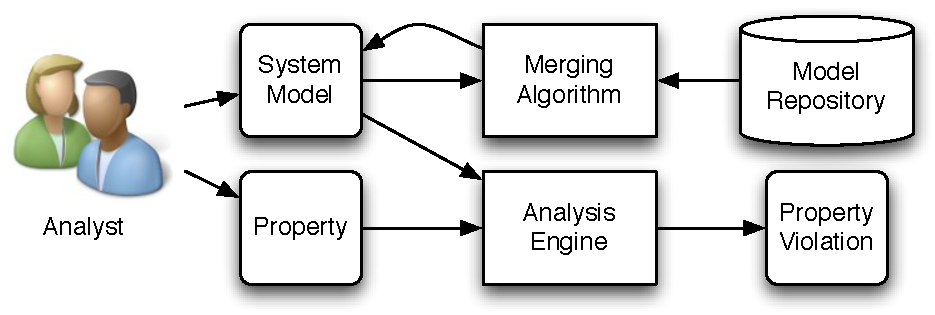
\includegraphics[width=0.60\textwidth]{diagrams/overview}
\caption{Overview of our framework on model construction and analysis.}
\label{fig-overview}
\end{figure}

In this paper, we propose a framework to aid the analyst in
incremental construction and analysis of a system model. The analyst
can use our framework to automatically augment an initial, high-level
design model with domain-specific knowledge, and uncover potential
violation of a property that may result from different design choices.

Our framework consists of three key components, as shown in
Figure~\ref{fig-overview}: (1) a repository of models that encode
common knowledge about the problem domain, (2) an algorithm that
merges two independent models of a system, and (3) an analysis engine
that checks whether a system model satisfies a given property, and if
not, produces a counterexample. In a typical workflow, the analyst
begins by constructing a partial model of the system, and runs an
initial analysis to check the system against a desired property. The
analyst then incrementally elaborates the initial model into a more
detailed one by \fix{merging it with the existing models in the
  repository, one-by-one}{selecting a set of existing models from the
  repository, relevant for the particular category of the system under
  design, and merging them into the initial one.  Each such model from
  the repository is written by a domain expert and encodes a piece of
  domain knowledge (e.g., feature, security threat, vulnerability,
  etc.) of an entire category of systems (e.g., networks, web
  applications, HTTP servers, etc.).}\am{it's probably not very
  important to say here that this is done one at a time; your tool
  could in principal merge many of them}. After every merge step, the
analyst re-runs the analysis on the elaborated model to detect any
potential violations that were absent from prior analyses.

A technical challenge in composing two independent models is that they
may not be amenable to composition due to \textit{abstraction
  mistmach}.\am{would it be worth noting here that the
  models are also declarative, written in logic, which also makes it
  difficult?} The two models may describe some aspect of the system
at different layers of abstraction, using different sets of vocabulary
terms, so standard composition techniques that connect components at
their interfaces may fail. To resolve this mismatch, we allow the
analyst to specify relationships between various parts of the two
models. Our merging algorithm then automatically constructs a new
model that is the result of composing two mismatched models according
to the specified relationships.

We do not aim to completely automate the model construction process;
our framework still relies on the analyst to use insights about the
system to drive the model elaboration process, and interpret the
output of the analysis engine to devise meaningful fixes to the
model. Our goal is to facilitate the model construction and analysis
process in the following ways:
\begin{itemize}
\item \textbf{Knowledge reuse}: A repository of generic domain models,
  constructed by a domain expert, can be reused for analysis of
  multiple systems. For example, a repository of models about common
  attacks on web applications may be used to analyze the security of
  multiple, independent web protocols.
\item \textbf{Incrementality}: Instead of having to come up with a
  complete, monolithic model of a system, the analyst can
  incrementally explore different aspects of the system, one at a
  time. For example, the analyst may rank the available attack models
  in the order of their criticality, and analyze the system for the
  most pressing issues first.
\item \textbf{Adaptiveness}: As the repository is updated with new
  models (e.g., newly discovered attacks or new operating environments),
  the analyst may repeat the analysis process without having to build
  the model from the scratch.
\end{itemize}

\textbf{Contributions} The contributions of this paper are as
follows:\am{small first letters in the following list?}
\begin{itemize}
\item a framework for incremental construction and analysis of a
  system model that leverages a domain-specific model repository,
\item a technique for merging two potentially mismatched models,
\item an implementation of the framework, including a language for
  specifying system models and an automated analysis engine built on
  top of a model finder, and
\item application of the framework to the analysis of two well-known
  web protocols, OAuth~\cite{oauth} and OpenID~\cite{openid}.
\end{itemize}

\textbf{Outline} This paper is structured as
follows. Section~\ref{sec-overview} provides an overview of our
framework with an example from an online news paywall system.
Section~\ref{sec-formalism} introduces our underlying formalism for
modeling systems. Section~\ref{sec-merging} describes the types of
relationships that the analyst can specify between two potentially
mismatched models, and the merging algorithm that composes the two
based on the given relationships. Section~\ref{sec-implementation}
discusses the implementation of the modeling formalism as a
domain-specific language as well as an automated analysis of merged
models. Section~\ref{sec-case-study} describes the case studies on
applying our approach to the OAuth and OpenID protocols. The paper
concludes by discussing the related work
(Section~\ref{sec-related-work}), and the potential benefits and
limitations of our approach (Section~\ref{sec-discussion}).

% However, there are a number of risks in reaching such a conclusion:
% (1) the analysis technique used may be unsound or incomplete, (2) the
% analyst may have specified an incorrect property, or (3) the model
% used in the analysis may (purposely or inadvertently) omit details
% about the system that, in reality, could lead to a violation of the
% property.


\section {Overview}
\label{sec-overview}

In this section, we give an informal overview of how an analyst would
use the framework to incrementally construct and analyze a model of a
system. We use an example from the web application domain to
illustrate our appraoch.

\paragraph{\textbf{Building an Initial Model}} Let us assume that the
\textit{New York Times}, a well-known news organization, wishes to
design a \textit{paywall} system for its online web site. A paywall
system is used to limit readers to a set number of free articles over
a time period, requiring them to signup for a paid subscription once
they reach the limit. One desirable property of this paywall
system is that \textit{readers who have already exceeded the limit
  should not be able to access an article}.

Alice, the chief web designer of the New York Times, devises a simple
design of the paywall system, as shown in
Figure~\ref{fig-nytimes}(a). There are three basic participants in this
design: the \textsf{NYTimes} server, which stores and serves articles,
\textsf{Reader}, an end-user who wishes to access an article, and
\textsf{Client}, which mediates the transfer of articles between
\textsf{NYTimes} and \textsf{Client}. When \textsf{Reader} selects a
link to an article, \textsf{Client} forwards the request for the
article to the \textsf{NYTimes} server, sending along a counter
(\textsf{currCounter}) that represents the number of articles
\textsf{Reader} has accessed so far. \textsf{NYTimes} accepts a
request \textsf{GetPage} from \textsf{Client} only if
\textsf{currCounter} is less than the limit. Once processing the
request, \textsf{NYTimes} then sends back a page that contains the
requested article, along with an increment of the original counter
(\textsf{newCounter}).

\begin{figure*}[!t]
  \centering \subfloat[NYTimes
  Paywall]{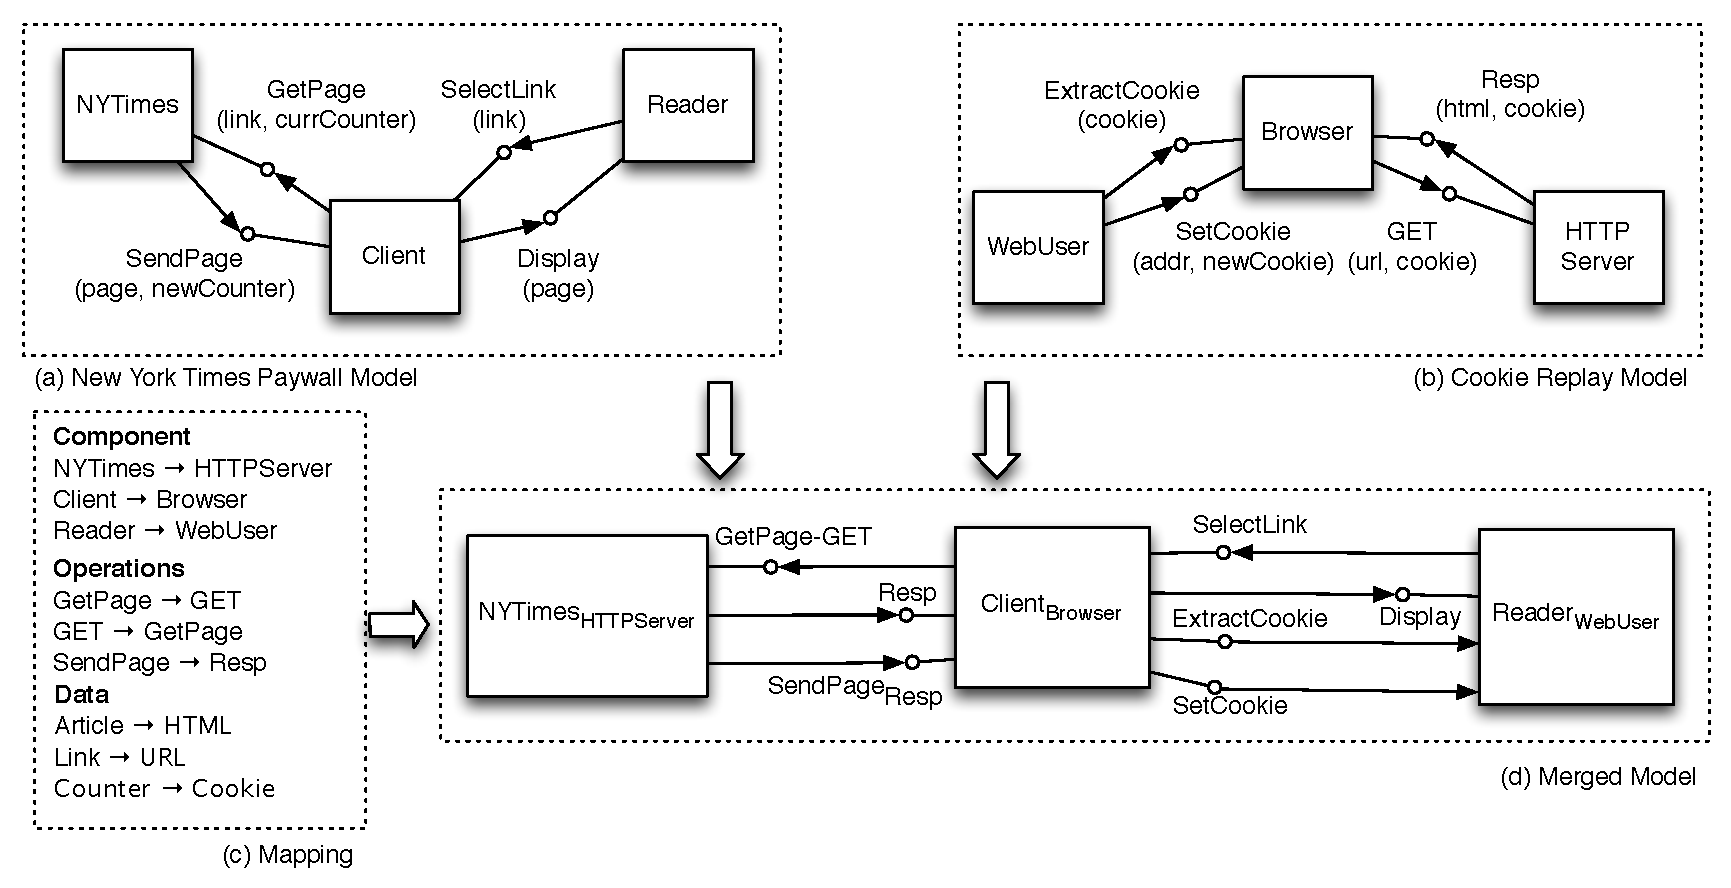
\includegraphics[width=0.48\textwidth]{diagrams/nytimes}}
  \hfil \subfloat[Cookie
  Replay]{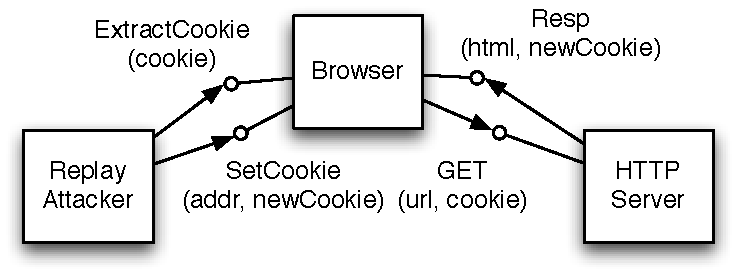
\includegraphics[width=0.51\textwidth]{diagrams/replay}}
\caption{Models of (a) the New York Times paywall system and (b)
  a cookie replay attack. A box represents a module, and a
  directed edge from one module \textsf{A} to another module
  \textsf{B} with label \textsf{O} represents \textsf{A}'s invocation
  of operation \textsf{O} that is exported by \textsf{B}.}
\label{fig-nytimes}
\end{figure*}

Note that the model in Figure~\ref{fig-nytimes}(a) describes the system
interactions in terms of web API operations. This level of abstraction
is suitable for the designer to capture the essential functionality of
the system; it omits low-level details that are irrelevant to the
system workflow, such as what kind of devices various participants
are deployed on, how various API operations are implemented, or the
type of data structure that is used to represent counters and pages.

To ensure that the design is satisfactory, Alice decides to run the
model in Figure~\ref{fig-nytimes}(a) through an analysis engine that
exhaustively explores the behavior of the model. As expected, the
engine concludes that the system satisfies the property by preventing
the reader from accessing an article beyond the limit.

\paragraph{\textbf{Elaborating the System Model}} Being satisfied with the
initial design, Alice moves onto exploring lower-level design
choices for the system. She decides that \textsf{NYTimes} will run on
top of an HTTP server, with \textsf{GetPage} implemeneted as a
standard HTTP GET operation. Similarly, she
designates \textsf{Client} to run on top of a standard web browser,
and the access counter to be stored as a cookie inside the browser.

Alice decides to explore the potential implications of these design
decisions on the security of the system using our framework. Let us
assume that the repository is already populated with models that
describe different types of attacks that are applicable to web-based
systems. For example, one type of attack that the paywall system might
be vulnerable to is a \textit{cookie replay attack}, which involves a
malicious user obtaining a cookie and repeating its transmission to a
server. In this model, shown in Figure~\ref{fig-nytimes}(b),
\textsf{Browser} communicates to \textsf{HTTPServer} by sending
\textsf{GET} requests and receiving responses (\textsf{Resp}) in
return. In addition, a malicious user (named \textsf{ReplayAttacker})
interacts with \textsf{Browser} by extracting a cookie from it
(\textsf{ExtractCookie}), or overwriting an existing cookie at a
particualr address (\textsf{SetCookie}); this allows
\textsf{ReplayAttacker} to manipulate \textsf{Browser} into sending a
request with a fixed cookie value.

A next step for Alice would be to extend the original paywall model
with new details from the cookie replay model, and re-run the analysis
to see whether the elaborated model still satisfies the desired
property. However, the two models, as in their current form, are not
readily amenable to composition due to an \textit{abstraction
  mismatch}. These models describe the system at different layers of
abstraction, using two distinct sets of vocabulary terms to describe
modules, operations, and data elements. They serve as \textit{partial}
descriptions of a system, including only the details of the system
that are necessary to illustrate a typical workflow (as in the paywall
model) or the characteristics of a particular attack (in the replay
model). Thus, additional guidance is needed to identify relationships
between parts of the two models before they can be merged.

Our observation is that relationships between a pair of models
correspond to the designer's decisions about how different parts of
the system are to be realized. For example, based on Alice's decisions
about the implementation of the paywall system, we may infer that
\textsf{NYTimes} and \textsf{HTTPServer} can be treated as the same
component; in particular, \textsf{NYTimes} can be considered a type of
\textsf{HTTPServer} that performs a specialized function of serving
articles to its client. A similar kind of relationship can be
specified between a pair of operations (e.g., \textsf{GetPage} and
\textsf{GET}) or data types (e.g, \textsf{Link} and \textsf{URL}). Given
the relationships specified by Alice, our framework merges the two
models and produces a new model that combines both aspects of the
system, as shown in Figure~\ref{fig-merged}.

\begin{figure}[!t]
\centering
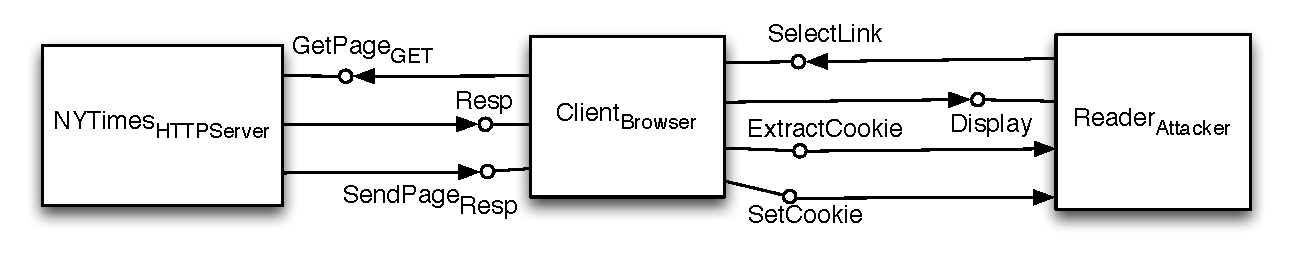
\includegraphics[width=0.9\textwidth]{diagrams/merged}
\caption{Result of merging the two models from
  Figure~\ref{fig-nytimes}. A subscript $Y$ in $X_{Y}$ implies that
  $X$ is a type of $Y$.}
\label{fig-merged}
\end{figure}

\paragraph{\textbf{Re-Analyzing the Model}}

Alice re-runs the analysis engine on the new, merged model to check
whethe the elaborated system still satisfies the desired
property. This time, the analysis engine discovers a counterexample
that demonstrates how the system might allow the reader to access an
article beyond the limit. In this scenario, \textsf{Reader}, now
acting like \textsf{ReplayAttacker}, extracts a cookie that represents
the access counter prior to reaching the limit. Then, \textsf{Reader}
simply overwrites the existing cookie with the extracted once the
limit is exceeded, and \textsf{NYTimes} continues to serve
\textsf{GetPage} requests from \textsf{Client}~\footnote{The actual
  paywall system for the New York Times suffered this type of attack
  when it was first introduced in 2008~\cite{nytimes-attack}.}. To
prevent this type of attack, Alice modifies the system such that when
\textsf{NYTimes} sends back a cookie, it generates and includes a
unique token that cannot be guessed by \textsf{Reader}, thereby
rendering old cookies invalid.

Alice may repeat the whole process again, elaborating the system model
with further details from other types of attack models in the
repository, and re-running the analysis engine to discover more
potential design flaws.


\section{Modeling Formalism}
\label{sec-formalism}

% Before describing how we reconcile the types of mismatch that we
% discussed in Section~\ref{sec-mismatch}, we first introduce the
% underlying formalism that is used for specifying systems, attacks, and
% security properties.
In this section, we describe, using a standard first-order logic, the
underlying formalism that our framework uses to specify a system and
its behavior. 

\paragraph{\textbf{Structure}} Figure~\ref{fig-formalism} summarizes
the basic constructs of our formalism. A system consists of a set of
\textit{components} $C$ that asynchronously communicate with each
other through \textit{operations} $O$. Each component \textit{exports} zero or
more operations at its interface, and \textit{stores} a set of
\textit{data} $D$. A piece of data $d \in D$ flows from component $c1$
to another component $c2$ when $c1$ \textit{invokes} $c2$'s operation
$o$ that includes $d$ as one of its \textit{arguments}. 

For example, consider a snippet of the New York Times paywall
model\footnote{For convenience, we use the dot (.)  notation to refer
  a field element by name; for example, $c.exports$ refers to the
  $exports$ field of component $c$.} in
Figure~\ref{fig-nytimes-spec}. Component \textsf{NYTimes} accepts
incoming requests for an article through \textsf{GetPage}, which
carries two named arguments: a link to an article (\textsf{``link''})
and a counter that represents the number of articles accessed so far
(\textsf{``currCounter''}). \textsf{NYTimes} responds to to
\textsf{Client} by invoking the latter's \textsf{SendPage} operation,
which carries the requested article and a new counter to be stored
inside the browser. \ek{was:this enables our system to accurately
  track data flows and automatically check standard information flow
  properties such as \textit{integrity} and \textit{confidentiality}}.

\begin{figure}[!t]
\fbox{
\begin{minipage}[t]{0.97\textwidth}
\begin{minipage}[t]{0.455\textwidth}
\begin{tabular}{@{\quad}l@{\quad}l}
\multicolumn{2}{l}{\textbf{Sorts}} \\
$C, O, D, M$                    & \\
$N, F$                          & \color{comment} // Name, Formula\\
\\
\multicolumn{2}{l}{\textbf{Model} ($M$)} \\
$comps : \mathcal P (C)$  & \color{comment} // components \\
$data : \mathcal P (D)$  & \color{comment} // data sets \\
\end{tabular}
\end{minipage}
\quad
\begin{minipage}[t]{0.455\textwidth}
\begin{tabular}{@{\quad}l@{\quad}l}
\multicolumn{2}{l}{\textbf{Component} ($C$)} \\
$exports : \mathcal P (O)$      & \color{comment} // exported ops \\
$invokes : \mathcal P (O)$      & \color{comment} // invoked ops \\
$stores : N \pfun \mathcal P (D)$            & \color{comment} // stored data \\
$guard : O \pfun F$ & \color{comment} // guards on ops \\
\multicolumn{2}{l}{\textbf{Operation} ($O$)} \\
$args : N \pfun \mathcal P (D)$       & \color{comment} // arguments \\
\end{tabular}
\end{minipage}
\end{minipage}
}
\fbox{
\begin{minipage}[t]{0.97\textwidth}
\begin{tabular}{@{\quad}l@{\quad}l}
  \multicolumn{2}{l}{\textbf{Auxiliary Functions}} \\
  $incoming(c) = {\{ o \in c.exports \;|\; c.guard(o) \}}$ \\
  $canAccess(c) = \{ d \in D \;|\; d \in ran(c.stores) \;\lor \exists o \in incoming(c) \cdot d \in
  ran(o.args)\} $ \\
  $outgoing(c) = {\{ o \in c.invokes \;|\; c.guard(o) \land ran(o.args) \subseteq
    canAccess(c)\}}$ \\
\end{tabular}
\end{minipage}
}
\caption{Basic constructs of our modeling formalism. $ran$ returns the
  range of a function.}
\label{fig-formalism}
\end{figure}

\begin{figure}[!t]
\fbox{
\begin{minipage}[t]{0.97\textwidth}
\textcolor{comment}{// definition of the \textsf{Paywall} model}

$\textsf{Paywall}.comps = \{\textsf{NYTimes}, \textsf{Client},
\textsf{Reader}\}, \textsf{Paywall}.data = \textsf{Article} \cup \textsf{Link} \cup
\textsf{Counter}$ 

\textcolor{comment}{// operations for \textsf{NYTimes}}

$\textsf{NYTimes}.exports = \textsf{GetPage}, \textsf{NYTimes}.invokes = \textsf{SendPage}$

$\textsf{GetPage}.args =
\{(\textsf{``link''}, \textsf{Link}),(\textsf{``currCounter''}, \textsf{Counter})\}$

$\textsf{SendPage}.args =
\{(\textsf{``page''}, \textsf{Article}),(\textsf{``newCounter''}, \textsf{Counter})\}$

$\textsf{NYTimes}.stores =
\{\textsf{(\textsf{``articles''}, \textsf{Map[Link,Article]})}\}$ 

\textcolor{comment}{// behavior of \textsf{NYTimes} with respect to
  its operations}

$\forall o \in \textsf{GetPage} \cdot \textsf{NYTimes}.guard(o) = f_1 $
where $f_1 \equiv o.args(\textsf{``currCounter''}) \leq \textsf{LIMIT}$

$\forall o \in \textsf{SendPage} \cdot \textsf{NYTimes}.guard(o) = f_2
$ where

$\quad f_2 \equiv \exists t \in \textsf{GetPage} \cdot t.args(\textsf{``page''}) =
\textsf{NYTimes}.stores(\textsf{``articles''})[t.args(\textsf{``link''})]
\land$ 

$\quad\quad\quad\quad\quad\quad\quad\quad\quad\quad o.args(\textsf{``newCounter''}) = t.args(\textsf{``currCounter''}) + 1$
\end{minipage}
}
\caption{A snippet of the New York Times paywall model. Assume that
  \textsf{Map[K, V]} is a predefined data type that represents a map
  from \textsf{K} to \textsf{V}; $m[k]$ returns the value stored in
  map $m$ at key $k$.}
\label{fig-nytimes-spec}
\end{figure}

Finally, a system model $m \in M$ is
simply defined as a set of components ($comps$) and data sets
($data$). 

\paragraph{\textbf{Behavior}} A component may not allow every incoming
operation, and may not send out arbitrary messages to other
components. For every instance of operation that it exports, the
component can impose a \textit{guard} constraint on the set of the
operations that it is willing to accept. For example, as defined in
Figure~\ref{fig-nytimes-spec}, \textsf{NYTimes} only accepts a request
for an article only if \textsf{currCounter} provided with the request
does not exceed the limit.

Similarly, a component may define a guard to restrict operations that
it can invoke, or impose a constraint on arguments that are carried
along with the invoked operations. For example, \textsf{NYTimes} may
invoke \textsf{SendPage} on the client only if it has already received
and accepted a valid \textsf{GetPage} message. In addition,
\textsf{SendPage} must include, as arguments, an article that
corresponds to the requested link, and an increment of the current
counter.  In effect, guard constraints are used to
declaratively specify the behavior of a component in terms of input
and output operations that it is allowed to perform.

The overall behavior of component $c$ is characterized by
$incoming(c)$ and $outgoing(c)$. Intuitively, $incoming(c)$ represents
the subset of incoming operations that are deemed valid and accepted
by $c$. Members of $incoming(c)$, in turn, determine the set of data
that $c$ can access; namely, $c$ can access a piece of data $d$ if and
only if $c$ already stores $d$, or $d$ flows into $c$ as part of a
valid incoming operation. Finally, $outgoing(c)$ represents the set of
invocations that $c$ is allowed to make; note that the arguments of $o
\in outgoing(c)$ are restricted to only those data elements that $c$
can access.

\paragraph{\textbf{Properties}} A desirable property about the system
can be expressed in terms of $incoming$, $outgoing$, and
$canAccess$. For example, the property for the paywall example can be
written as
\begin{align*}
\# canAccess(\textsf{Reader}) \leq \textsf{LIMIT}
\end{align*}
where $\# S$ returns the cardinality of set S. An ensuing analysis
would then attempt to check whether the guards specified in the
components are strong enough to establish the property, and if not,
produce an instance of $canAccess$ that contradicts the above
constraint. 

%\begin{figure}[ht]
\centering
  \begin{slangmath}[frame=single]
    view Paywall

    Paywall.data = {Page, Link}
    Paywall.mods = {NYTimes, Client, Reader}

    NYTimes.exports = {GetPage}
    NYTimes.invokes = {SendPage}
    NYTimes.stores  = {"articles" -|-> Map[Link, Page]}
    NYTimes.cons    = {??}

    // similar for Client and Reader

    GetPage.args = {"link" -|-> Link, "currCounter" -|-> Int}
  \end{slangmath}

\caption{Formal specification of the Paywall example.}
\label{fig-paywall-formal}
\end{figure}



\section{Technique for Merging Models}
\label{sec-merging}

In this section, we describe a technique for merging two potentially
mismatched models that describe different aspects of a system. The
merging process is two-fold. First, the analyst specifies the
relationship between two models as a mapping between different
entities in them. Then, given this mapping, we apply an algorithm to
produce a merged model with potentially new behaviors that arise
from the interaction of the components from the previously separate
models.

\subsection{Specifying Relationships between Models}
\label{sec-relationship}

To resolve potential mismatch between two models, the analyst may
specify a relationship between a pair of components, operations, or data
elements. Our notion of a relationship between two entities is that of
a \textit{subset} relation. Informally, two entities are related if
they both describe the same concept in the real world, but one is a
generic representation of the other. \ek{For example,
\txtcname{NYTimes} can be regarded as a specialized kind of
\txtcname{HTTPServer} with the role of controlling access to articles
that it stores.  A similar kind of relationship can be introduced
between operations or data elements. Operation \txtcname{GetPage},
implemented using a generic HTTP request, can be regarded as a kind of
\txtcname{GET} operation. Similarly, since a counter is stored as a
cookie, \txtcname{Counter} can be treated as a kind of \txtcname{Cookie}.}

\begin{defn} A relationship $r \in R$ between two models is a tuple
  $(r_{C}, r_{O}, r_{D})$ where $r_{C} \subseteq C \times C$, $r_{O}
  \subseteq \mathcal P (O) \times \mathcal P (O)$, and $r_{D}
  \subseteq \mathcal P (D) \times \mathcal P (D)$ represent subset
  relations between a pair of components, operation sets, and data
  sets, respectively.
\end{defn}
For example, to merge the paywall and cookie replay models from
Figure~\ref{fig-nytimes}, Alice may specify the following
relationships between the two models:
\begin{scriptsize}
\begin{align*}
  r_{C} = \{&(\txtcname{Client$,$ Browser}),(\txtcname{NYTimes$,$
    HTTPServer}), (\txtcname{Reader$,$
    WebUser})\} \\
  r_{O} = \{&(\txtcname{GetPage$,$ GET}), (\txtcname{GET$,$ GetPage}),
  (\txtcname{SendPage$,$
    Resp})\}\\
  r_{D} = \{&(\txtcname{Article$,$ HTML}),(\txtcname{Link$,$ URL}),
  (\txtcname{Counter$,$ Cookie})\}
\end{align*}
\end{scriptsize}
A subset relation is asymmetrical, and so two entities can be
specified as equivalent by including a tuple and its inverse in the
same relation; for example, $r_{O}$ here specifies that
\txtcname{GetPage} operations are the only kind of \txtcname{GET}
operations that will be exported by \txtcname{NYTimes} running on top of
a HTTP server.

% Intuitively, these relationships correspond to the system designer's
% decisions about how components, operations, and data are to be realized
% and implemented. By varying these relationships, the designer can
% explore the security implications of different design decisions. For
% example, in another variation of OAuth, the designer may decide to
% deploy \txtcname{Client} as a server-side application instead of a
% client-side application running on the top of a browser; in this
% case,\txtcname{Client} and \txtcname{TrustedServer} would be specified as
% an entry in $r_{M}$. As a consequence of this relationship,
% \txtcname{Client} would inherit the characteristics of
% \txtcname{TrustedServer}, and now be susceptible to server-side attacks
% instead of browser-based ones.

\begin{algorithm}[t!]
\begin{algorithmic}[1]
\hskip-20pt
\begin{minipage}[t]{0.60\linewidth}
\Function{MergeModels}{$m_{1}, m_{2}, r$}
\Let{$h$}{\textsf{MkMap}($m_{1}$, $m_{2}$, $r$)}
\Let{$m'$}{\textsf{MkModel}($m_{1}$, $m_{2}$, $h$)}
%\Let{$m'$}{\textsf{Substitute}}($m'$, $h$)
\State \Return{$m'$}
\EndFunction

\item[]
\Function{MkMap}{$m_{1}, m_{2}, (r_{C}, r_{O}, r_{D})$}
\ForAll{$(D_{1}, D_{2}) \in r_{D}$}
\Let{$h_{D}(D_{1})$}{\textsf{MergeData}($D_{1}$, $D_{2}$)}
\EndFor
\ForAll{$(c_{1}, c_{2}) \in r_{C}$}
\Let{$h_{C}(c_{1}), h_{C}(c_{2})$}{\textsf{MergeComp}($c_{1}$, $c_{2}$, $r_{O}$)}
\EndFor
\State \Return{$(h_{C}, h_{D})$}
\EndFunction

\item[]
\Function{MkModel}{$m_{1}, m_{2}, (h_{C}, h_{D})$}
\Let{$C', D'$}{$\varnothing$}
\ForAll{$m \in m_{1}.comps \cup m_{2}.comps$}
\If{$m \in dom(h_{C})$}
\Let{$C'$}{$C' \cup \{h_{C}(m)\}$}
\Else
\Let{$C'$}{$C' \cup \{m\}$}
\EndIf
\EndFor
\ForAll{$ds \subseteq m_{1}.data \cup m_{2}.data$}
\If{$ds \in dom(h_{D})$}
\Let{$D'$}{$D' \cup h_{D}(ds)$}
\Else
\Let{$D'$}{$D' \cup ds$}
\EndIf
\EndFor
\State \Return{$(C',D')$}
\EndFunction

\item[]
\Function{MergeData}{$D_{1}, D_{2}$}
\Let{$f_{D_{1},D_{2}}$}{\textsf{MkEmbeddingFunc}($D_{1}$, $D_{2}$)}
\Let{$D'$}{$f_{D_{1},D_{2}}(D_{1})$}
\State \Return{$D'$}
\EndFunction
\end{minipage}
\quad
\begin{minipage}[t]{0.55\linewidth}
\item[]
\Function{MergeComp}{$c_{1}, c_{2}, r_{O}$}
\Let{$e, i$}{$c_{2}.exports, c_{2}.invokes$}
\Let{$s, g$}{$c_{1}.stores \cup c_{2}.stores, c_{1}.guard \cup c_{2}.guard$}
\ForAll{$(O_{1}, O_{2}) \subseteq c_{1}.exports \times c_{2}.exports$}
\If{$(O_{1}, O_{2}) \in r_{O}$}
\Let{$e$}{$e \cup \textsf{MergeOp}(O_{1}, O_{2})$}
\Else
\Let{$e$}{$e \cup O_{1}$}
\EndIf
\EndFor
\ForAll{$(O_{1}, O_{2}) \subseteq c_{1}.invokes \times c_{2}.invokes$}
\If{$(O_{1}, O_{2}) \in r_{O}$}
\Let{$i$}{$i \cup \textsf{MergeOp}(O_{1}, O_{2})$}
\Else
\Let{$i$}{$i \cup O_{1}$}
\EndIf
\EndFor
\Let{$c'$}{$(e,i,s,g)$}
\State \Return{$c'$}
\EndFunction

\item[]
\Function{MergeOp}{$O_{1}, O_{2}$}
\Let{$f_{O_{1},O_{2}}$}{\textsf{MkEmbeddingFunc}($O_{1}$, $O_{2}$)}
\Let{$O'$}{$f_{O_{1},O_{2}}(O_{1})$}
\ForAll{$o \in O_{1}$} \Let{$f_{O_{1},O_{2}}(o).args$}{$f_{O_{1},O_{2}}(o).args \cup o.args$}
\EndFor
\State \Return{$O'$}
\EndFunction

% \item[]
% \Function{Substitute}{$v, (h_{m}, h_{D})$}
% \State ... // Omitted
% \State \Return{$v$}
% \EndFunction
\end{minipage}

\end{algorithmic}
\caption{Merging Models}
\label{alg-merge-models}
\end{algorithm}


\begin{figure}[ht]
\hrule\hrule
\centering
  \begin{slangmath}[numbers=left,emph={MergeModels, MkMap, MkModel,%
                    MergeData, MergeComp, MergeOp, MapSum}]
fun MergeModels($m_1, m_2, (r_c,r_O,r_D)$)
  let $h_D=$ map(($\lambda D_1,D_2 \cdot$($D_1,$MergeData($D_1, D_2$))), $r_D$)
  let $h_C=$ map(($\lambda C_1,C_2 \cdot$ let $C'=\; $MergeComp($C_1, C_2$) in [$(C_1, C'),\; (C_2, C')$]), $r_C$)
  MkModel($m_1, m_2, h_C, h_D$)

fun MkModel($m_1, m_2, h_C, h_D$)
  let $f_{map} = \lambda h,e \cdot (e \in dom(h)) \;?\; \{h[e]\} : \{e\}$
  (MapSum($m_1.comps \cup m_2.comps,\; f_{map}(h_C)$), MapSum($m_1.data \cup m_2.data,\; f_{map}(h_D)$))

fun MergeData($D_1, D_2$)       \eqv MkEmbeddingFunc($D_1, D_2$)($D_1$)
fun MergeOp($O_1, O_2$)         \eqv let $O'=\; $MkEmbeddingFunc($O_1, O_2$)($O_1$)
                        $O'.args= O_1.args \cup O_2.args$ 
                        $O'$
fun MergeComp($c_1, c_2, r_O$)$\:$\eqv let $f_{map} = \lambda O_1,O_2 \cdot (O_1,O_2)\in r_O\;?\;$MergeOp($O_1,O_2$)$\;: O_1$
                        let $e = c_2.exports\;\cup\;$MapSum($c_1.exports \times c_2.exports,\; f_{map}$)
                        let $i = c_2.invokes\;\cup\;$MapSum($c_1.invokes \times c_2.invokes,\; f_{map}$)
                        $(e,\; i,\; c_1.stores \cup c_2.stores,\; c_1.guard \cup c_2.guard)$
fun MapSum($set, f_{map}$)          \eqv fold(($\lambda a, e \cdot a \cup e),\; \{\},\; f_{map}(set)$)
  \end{slangmath}
\hrule\vskip7pt
\caption{Algorithm for merging two models ($m_1$ and $m_2$) given a
  mapping ($r_C, r_O, r_D$).  The algorithm make use of the
  \slangmathinscript|MkEmbeddingFunc($set_1, set_2$)| function (which
  computes an embedding of $set_1$ into $set_2$ and returns a 1-arg
  function for mapping elements of $set_1$ to elements of $set_2$), as
  well as two standard library functions,
  \slangmathinscript|map($\lambda_{map},\; set$)| and
  \slangmathinscript|fold($\lambda_{fold},\; init,\; set$)|.}
\label{fig-merge-models-func}
%\label{alg-merge-models}
\end{figure}


\subsection{Merging Algorithm}

The algorithm for merging, shown in Algorithm~\ref{alg-merge-models},
accepts two models, $m_{1}, m_{2} \in M$, and a relationship $r \in R$
between them, and produces a new model, $m' \in M$. The algorithm is
divided into two steps. First, for every pair of entities $e1$ and
$e2$ specified in $r$, it merges them into a single entity $e'$ that is a
subset of $e2$, and corresponds to $e1$ (Line 2). Then, the algorithm
builds a new model by replacing every $e1$ in $r$ with $e'$ (Line 3).

% \begin{figure*}[!t]
% \centering
% \includegraphics[width=0.95\textwidth]{diagrams/oauth-csrf-merged}
% \caption{Result of Merging the OAuth and CSRF models from Figure~\ref{fig-oauth}.}
% \label{fig-merged-oauth-csrf}
% \end{figure*}

\subsubsection{Step 1: Merging Related Entities}

Procedure \txtcname{MkMap} performs the task of merging individual
entities in two-fold, first merging each pair of related data sets
(Line 7), and then merging the related components (Line
9). As output, \txtcname{MkMap} returns a pair of functions
($h_{C}$ and $h_{D}$) that map the original components and data sets
from $r$ to their merged counterparts; these functions are then used
in Step 2 to construct a merged model.

% \begin{figure}[!t]
% \centering
% \includegraphics[width=0.40\textwidth]{diagrams/embedding}
% \caption{Embedding of \textsf{Token} into \textsf{String}}
% \label{fig-embedding}
% \end{figure}

\paragraph{\textbf{Merging Data}} For each pair of data sets $(D_{1},
D_{2})$ in $r_{D}$, \textsf{MergeData} produces a new set of data, $D'$,
that replaces $D_{1}$ in the merged model $m'$, and can be treated
like instances of $D_{2}$. 

For example, given $(\txtcname{Article}, \txtcname{HTML}) \in r_{D}$, \txtcname{MergedData} produces a new data set $\txtcname{Article}_{\textsf{HTML}}$, which conceptually represents the encodings of the New York Times articles in HTML format. $\textsf{Article}$ and $\textsf{Article}_{\textsf{HTML}}$ correspond one-to-one; for every $a \in \textsf{Article}$, there exists a unique $a' \in \textsf{Article}_{\textsf{HTML}}$ such that $a'$ represents an HTML encoding of $a$. Note that there may be some HTML documents that do not correspond to any article (i.e., $\textsf{Article}_{\textsf{HTML}}$ is a strict subset of $\textsf{HTML}$).

Formally, $D'$ represents the result of \textit{embedding} $D_{1}$ into
$D_{2}$. Since members of $D_{1}$ and $D_{2}$ are abstract values, we can
construct an injective function $f : D_{1} \rightarrow D_{2}$ by assigning
to each $d_{1} \in D_{1}$ a unique counterpart $d_{2} \in D_{2}$. Then, an
embedding of $D_{1}$ into $D_{2}$ is simply the set $f(D_{1})$. For example,
let $f_{(\textsf{A,H})}$ be an embedding function that maps each
article to its HTML counterpart. Then, every $a \in \textsf{Article}$
in the original model $m_{1}$ can be substituted by
$f_{(\textsf{A,H})}(a)$ in the merged model $m'$.

% \begin{thm} For every $D_{1}, D_{2} \subseteq D$, there always exists a
%   function $f : D_{1} \rightarrow D_{2}$ such that f is an embedding from
%   $D_{1}$ to $D_{2}$.
% \end{thm}
% \todo{need proof here}
% \begin{proof} Omitted.
% \end{proof}

\paragraph{\textbf{Merging Components}} Given a pair of components
$(c_{1}, c_{2}) \in r_{C}$, along with pairs of related operations $r_{O}$,
\textsf{MergeComp} produces a new component $c'$ that combines the
behavior of $c_{1}$ and $c_{2}$.

The behaviors of the two components may be related through one or more
pairs of operations specified in $r_{O}$. If $c_{1}$ exports or invokes
a set of operations $O_{1}$ that are related to another set of operations
$O_{2}$ in $c_{2}$, \textsf{MergeComp} merges the two sets by using the
procedure \textsf{MergeOp}. 


\paragraph{\textbf{Merging Operations}} Operations are merged in the
similar fashion as the data elements; an embedding is used to
establish a subset relation between $O_{1}$ and $O_{2}$, resulting in a new
set of operations $O' \subseteq O_{2}$, which also inherits all of the
arguments from $O_{1}$ and $O_{2}$ (Line 47).

For example, given $(\txtcname{SendPage}, \txtcname{Resp}) \in r_{O}$,
$MergeOp$ produces $\txtcname{SendPage}_{\textsf{Resp}}$, which
represents the implementation of \txtcname{SendPage} as a standard HTTP
response.  $\txtcname{SendPage}_{\textsf{Resp}}$ can be used by
\txtcname{NYTimes} to send an article back to
$\txtcname{Client}_\textsf{Browser}$, but is also treated like any
standard HTTP response. Note that $\txtcname{Client}_\textsf{Browser}$
may receive other kinds of HTTP responses besides the ones that carry
an article from \txtcname{NYTimes}; i.e., there may exist $r \in
\txtcname{Resp}$ that is not a member of $\txtcname{SendPage}_{\textsf{Resp}}$.

The guard function of the merged component $c'$ is constructed
as the union of $c_{1}.guard$ and $c_{2}.guard$ (Line 30). This ensures that $c'$
maintains the behaviors of both $c_{1}$ and $c_{2}$ with respect to the
operations that they export and invoke, including the merged
operations. To be more precise, the set of constraints applicable to $o' =
MergeOp(O_{1}, O_{2})$ can be characterized as follows:
\begin{align*}
c'.guard(o') = \bigwedge \{& l \in F \;|\; l \in c_{2}.guard(o') \; \lor \\
&\exists o1 \in O_{1} 
\cdot o' = f_{O_{1}, O_{2}}(o1) \land l \in c_{1}.guard(o1) \} 
\end{align*}
In other words, since $o'$ can be considered a member of both $O_{1}$ and
$O_{2}$, $o'$ retains all of the constraints that $c_{1}$ and $c_{2}$ impose
on $O_{1}$ and $O_{2}$, respectively. 

Finally, the set of data that $c'$ stores is constructed as the union
of $c_{1}.stores$ and $c_{2}.stores$ (Line 30).

\todo{example with invokes constraints on SendResp}

\todo{Explain why Alice specified GET and GetPage to be equivalent}

\ek{ \paragraph{\textbf{Remarks}} Note that the merging algorithm
does not enforce any constraint between the arguments of two
operations being merged, or the fields of two data sets. Say
this was intentionally done to make the mapping lightweight}

% To be more precise about what it means for a component to behave like
% another, we use the notion of observational refinement that we
% introduced earlier:
% \begin{thm}
% \label{thm-refinement}
% Given $r \in R$ and $(m_{1}, m_{2}) \in r_{M}$, let $m' = MergeComp(m_{1},
% m_{2}, r_{O})$. Then, $m'$
% is an observation refinement of both $m_{1}$ and $m_{2}$.
% \end{thm}
% \begin{proof}
%   By construction, for every operation $o \in O$ in $m'$ that
%   originated from $m_{1}$, $m'$ retains all of the constraints on $o$
%   from $m_{1}$ (i.e., $m_{1}.cons(o) \subseteq m'.cons(o)$). Thus, $m'.in$
%   and $m'.out$ are subsets of $m_{1}.in$, and $m_{1}.out$, respectively,
%   satisfying the conditions for an observational refinement of $m_{1}$ by
%   $m'$.  Similarly, since $m'$ retains all of the constraints on every
%   operation that it inherits from $m_{2}$, $m'$ is an observational
%   refinement of $m_{2}$.
% \end{proof}
% The key intuition behind the proof is that the merging operation only
% restricts the behaviors of the components on merged operations, and
% retains the same behaviors for all other operations. For example, from
% \txtcname{Client}'s perspective, the merged component
% $\txtcname{AuthorizationServer}_\textsf{TS}$ still behaves like
% \txtcname{AuthorizationServer}, receiving
% requests and sending back an access token only if a valid credential
% is provided.

\subsubsection{Step 2: Mking a New Model}

Once the different parts of the models have been merged according to
the given relationships, constructing the merged model is a
straightforward process. Using the function $h_{C}$ that maps a component
from an existing component to its merged counterpart, \txtcname{MkModel}
simply replaces each of the components that appear in $r_{C}$ with the
new merged one (Line 15), while leaving those that do not appear in
$r_{C}$ intact (Line 17). Similarly, \txtcname{MkModel} uses $h_{D}$
to replace each of the data sets from $m1$ that appears in $r_{D}$
with its embedded counterpart (Line 20).  

\subsection{Implications of Merging}

Merging two models introduces a new set of behaviors into
the original model of the system, some of which may lead a violation
of a property that prior analyses might have ruled out. We categorize
different types of interactions that arises as a result of
merging. Let $c_1, c_2 \in C$ be components from models $m_{1}$ and
$m_{2}$, $D_1, D_2 \subseteq D$ be data sets from $m_{1}$ and $m_{2}$, and
$O_1, O_2 \subseteq O$ be the sets of operations that $c_1$ and $c_2$
exports, respectively. 

\textbf{A merged component exports additional operations}. Let $c'$ be
the result of merging $c_1$ with $c_2$. Then, $c'$ exports operations
$O_2$, which are absent from $m_1$, introducing new interactions
between $c_1$ and the invokers of $O_2$ in $m_2$. Going back to the
New York Times example in Figure~\ref{fig-nytimes}, by being merged
with \textsf{Browser}, \textsf{Client} obtains two additional
operations, \textsf{ExtractCookie} and \textsf{SetCookie}, allowing
$\textsf{Reader}_\textsf{WebUser}$ to manipulate the counter stored in
$\textsf{Client}_\textsf{Browser}$.

\textbf{A merged operation is invoked by additional components}. Let $O'$
be the result of embedding $O_1$ into $O_2$. Then, $O'$ may be invoked
by all components in $m_2$ that invoke $O_2$, introducing new interactions
between $c_1$ and the invokers of $O_2$ in $m_2$. By being merged with
\textsf{GET}, \textsf{GetPage} becomes a kind of HTTP GET operations;
this means that, for example, any component that invokes \textsf{GET}
may also invoke $\textsf{GetPage}_\textsf{GET}$.

\textbf{A merged data element is included as arguments in additional
  operations.}  Let $D'$ be the result of embedding $D_1$ into
$D_2$. Then, for some $O_2$ that expects an argument $a \in D_2$, a
member of $D'$ may also be substituted for $a$, introducing new flows
of data $D_1$ to the exporters of $O_2$ in $m_2$. Since
$\textsf{Counter}_\textsf{Cookie}$ is now a subset of
$\textsf{Cookie}$, a counter can be provided as the $\textsf{cookie}$
argument in $\textsf{ExtractCookie}$.

It may be a combination of one or more of the above interactions that
lead to a property violation. For example, it is
$\textsf{Reader}_\textsf{WebUser}$ being able to set a cookie inside
$\textsf{Client}_\textsf{Browser}$, combined with the design decision
that a \textsf{Counter} be stored as a \textsf{Cookie}, that allows
the reader to access an article beyond the limit. Then, the task of
the analysis engine is to consider all combinations of interactions
that arise from merging and check whether any one of them could lead
to a violation.

% One
% consequence of the merging is that there are new interactions among
% components that did not exist before. For example, the malicious server
% now interacts with the client application by receiving and sending
% HTTP messages.

% Figure~\ref{fig-merged-oauth-csrf} shows the result of merging the
% OAuth and CSRF models from Figure~\ref{fig-oauth} according to the
% relationships that we specified in Section~\ref{sec-relationship}.
% One example of a CSRF attack against OAuth, made possible due to new
% interactions in the merged model, is as follows. The goal of the
% attacker is to trick the resource owner into granting more resources
% to the client than would be normally desirable by him or her (for
% example, granting write access to the entire Facebook profile, instead
% of just read access). The attack begins when
% $\txtcname{ResourceOwner}_\textsf{EndUser}$ visits a URI that is owned
% by \txtcname{MraliciousServer}, which, then crafts a DOM that is designed
% to force $\txtcname{Client}_\textsf{B}$ into sending
% $\txtcname{reqAccessToken}_\textsf{hreq}$ to
% $\txtcname{AuthorizationServer}_\textsf{TS}$. In particular, this
% request is constructed so that it includes, for argument
% $\txtcname{resID}$, some $\txtcname{badResID}$ $\in$ $\txtcname{ResourceID}$
% that identifies the resource that the attacker wishes to access.

% $\txtcname{Client}_\textsf{B}$, having inherited the behavior of
% \txtcname{Browser}, includes any associated cookies as part of the
% request headers. Since a cookie can be used as a credential,
% $\txtcname{AuthorizationServer}_\textsf{TS}$ accepts this request to be
% valid, and sends back the access token that corresponds to
% $\txtcname{badResID}$, giving $\txtcname{Client}_\textsf{B}$ full access
% to the resource. Note that the attacker was able to bypass the usual
% interactions between $\txtcname{Client}_\textsf{B}$ and
% $\txtcname{ResourceOwner}_\textsf{ES}$ and obtain an access token
% without first gaining permission from the resource owner.


\section{Implementation}
\label{sec-implementation}

To implement our approach, we (1) designed a domain-specific surface
language (called \sLangLong), and (2) wrote a compiler that translates
models written in \sLang to first-order relational logic (namely the
Alloy language~\cite{alloy}), which is amenable to fully automated
(but bounded) analysis~\cite{kodkod}.

The main design goal of \sLang is to provide a high-level paradigm for
writing formal system designs (architectures) which is intuitive and
readily accessible to analysts not already experienced in formal
methods.  \sLang, therefore, intentionally hides most of the internal
complexities of our declarative formalism; instead, \sLang provides a
mostly imperative service-oriented paradigm, which allows the analyst
to express valid system behaviors simply by specifying service
invocations that different components may perform.  Furthermore,
\sLang is fully embedded in Ruby (all \sLang programs are
syntactically correct Ruby programs), making the extensive set of
existing development tools for Ruby readily available, as well as
making the learning curve less steep.

In this paper, we do not attempt to evaluate the assertions about the
language simplicity and accessibility to non-experts in formal
methods; instead, we invite the community to contribute our existing
knowledge database by downloading \sLang~\cite{slang-web} and
submitting attack models in their domain of expertise.\check{!}

\subsection{The \sLang Language}
\begin{figure}[ht]
\centering
  \begin{slang}
view :Paywall do
  critical data Page
  data Link
  
  trusted component NYTimes [articles: Int ** Page, limit: Int] do
    creates Article
    operation GetPage [link: Link, currCounter: Int] do
      guard { currCounter < limit) }
      sends { Client::SendPage[articles[link]] }
    end
  end

  trusted component Client [counter: Int] do
    operation SendPage[article: Article] do 
      sends { Reader::Display[article] }
    end
    operation SelectLink[link: Link] do
      sends { NYTimes::GetPage[link, counter] }
    end
  end

  component Reader do
    operation Display[page: Page]
    sends { Client::SelectLink }
  end
end
  \end{slang}

\caption{Paywall example in \sc{Slang}}
\label{fig-paywall-slang}
\end{figure}


\Figref{fig-paywall-slang} shows the implementation of the running
``New York Times Paywall'' example in \sLang.  The main concepts from
our formalism (views, data, components, and operations) are specified
in \sLang by using a pseudo-keyword the same name\footnote{All
  pseudo-keywords in \sLang are implemented as plain Ruby methods}
(e.g., lines 1, 2, 3, 5, 7, etc.).  The containment relation between
them is implicitly defined by the nesting level, much like in Ruby and
the traditional object oriented programs in general.  For instance,
the call to the \bcode{view} function (line 1) defines the
\code{Paywall} view containing all the definitions inside the
\bcode{do ... end} block.  Component definitions can be prepended with
the \bcode{trusted} pseudo-keyword (lines 5, 13) to distinguish
trusted from potentially malicious components (if not explicitly
marked as trusted, the component is considered malicious, e.g., line
22).  Similarly, data definitions can be prepended with
\bcode{critical} (line 2); one of the predefined properties in our
framework checks that no critical data ever flows to a non-trusted
component.  The same syntax (a comma-separated list of
name$\rightarrow$type pairs between square brackets, i.e., a hash in a
singleton array in Ruby terms) is used to specify the data stored in
components (lines 5, 13) and operation arguments (lines 7, 14, 23).
Operations can have guards and responses: the former specifies a
precondition which must hold in order for the operation to be allowed
(e.g., line 8, only when the given argument (\code{currCounter}) is
less than the stored limit (\code{limit})), and the latter specifies
which operations and under what conditions the component invokes
whenever this operation is triggered.


\section{Case Study}
\label{sec-case-study}

We demonstrate that our framework can be used to incrementally explore
design alternatives for a web application and analyze their
implications on the security of the system. Types of design decisions
in the web application domain include:
\begin{itemize}
\item Authentication mechanism: Passwords, certificates,
  Kerberos, or more advanced protocols such as OpenID and OAuth.
\item Critical resource storage: Decisions about (1) where to store a
  piece of critical data (e.g., store a user session on the client vs
  server side), and (2) how to store it (in plain text vs encrypted).
\item Data transfer protocols: Mechanisms to transfer a piece of data
  between its components and protect it from malicious users (e.g,
  SSL vs TLS).
\item Deployment architecture: Decisions about the type of device onto
  which a component will be deployed (e.g., browser vs mobile app).
\item Implementation languages: The choice of a programming language
  used to implement a particular component.
\end{itemize}
Each decision may introduce different types of vulnerabilities into
the system. Furthermore, one or more of these decisions interact with
each other in subtle ways.

We have constructed a repository that contains models of these design
alternatives and their associated vulnerabilities. We have applied our
framework to analyze the design of several web applications \ek{what
  are these?}. For each of the applications, we began by building an
intiial model of a system that described the core system functionality
along with a desired security property, but omitted low-level design
decisions. We manually extracted the actual design choices of the
application, and incrementally added them to the model, each time
running our analysis engine to check whether the system might be
vulnerable to a security attack. When the analysis engine generated a
counterexample, we manually confirmed that it indeed represented a
real vulnerability by replaying a concretized version of the
counterexample on the system. In the following section, we report on
the vulnerabilities that we discovered in these applications, and on
the performance of the analysis engine.


 
\section{Related Work}
\label{sec-related-work}

TBD


\section{Discussion}
\label{sec-discussion}

TBD


%
% ---- Bibliography ----
%
%\begin{thebibliography}{0}
%
% \bibitem {clar:eke}
% Clarke, F., Ekeland, I.:
% Nonlinear oscillations and
% boundary-value problems for Hamiltonian systems.
% Arch. Rat. Mech. Anal. 78, 315--333 (1982)

% \bibitem {clar:eke:2}
% Clarke, F., Ekeland, I.:
% Solutions p\'{e}riodiques, du
% p\'{e}riode donn\'{e}e, des \'{e}quations hamiltoniennes.
% Note CRAS Paris 287, 1013--1015 (1978)

% \bibitem {mich:tar}
% Michalek, R., Tarantello, G.:
% Subharmonic solutions with prescribed minimal
% period for nonautonomous Hamiltonian systems.
% J. Diff. Eq. 72, 28--55 (1988)

% \bibitem {tar}
% Tarantello, G.:
% Subharmonic solutions for Hamiltonian
% systems via a $\bbbz_{p}$ pseudoindex theory.
% Annali di Matematica Pura (to appear)

% \bibitem {rab}
% Rabinowitz, P.:
% On subharmonic solutions of a Hamiltonian system.
% Comm. Pure Appl. Math. 33, 609--633 (1980)
%\end{thebibliography}

%\bibliographystyle{splncs}
\bibliographystyle{abbrv}
\bibliography{main}

\end{document}

